\label{chapter:sherifftools}

False sharing is a well-known performance issue~\cite{falseshare:effect, falseshare:Analysis}. We have discussed this problem in Section~\ref{sec:falsesharingproblems}. 

Detecting false sharing requires tools support. Existing tools share a similar shortcoming, where they can not pinpoint the exact place with false sharing problems, leaving the burden of finding actual places to programmers. Besides that, existing tools suffer from one or more different shortcomings.  Simulation based approaches ~\cite{falseshare:simulator} and binary instrumentation based approaches~\cite{falseshare:binaryinstrumentation1, falseshare:binaryinstrumentation2} normally introduce very significant performance overhead, slowing down the execution over $100\times$. Hardware performance counter based approaches generally provide much better performance, but they cannot differentiate false sharing from true sharing problems~\cite{detect:ptu, detect:intel}.

We provide two systems, \SheriffDetect{} and \SheriffProtect{}, to tackle with false sharing problems, based on the \sheriff{} framework that discussed in Section~\ref{sec:sheriffframework}. \Sheriff{} is a drop-in replacement of the standard \pthreads{} library, but providing ``per-thread'' protection and isolation mechanism. \SheriffDetect{} detects false sharing problem accurately (without false positives) and precisely, by pointing out the exact places with false sharing problems. It is also very efficient, only introducing 20\% performance overhead.  \SheriffProtect{} automatically tolerate false sharing problems when rewriting an application to resolve false sharing is infeasible or impractical. The reasons can be caused by either source code is unavailable, or padding data structures would degrade performance because of reduced cache utilization and/or increase memory footprint.


%\section{\sheriff{} Framework}
%\label{sec:overview}

\begin{figure*}[!t]
\centering
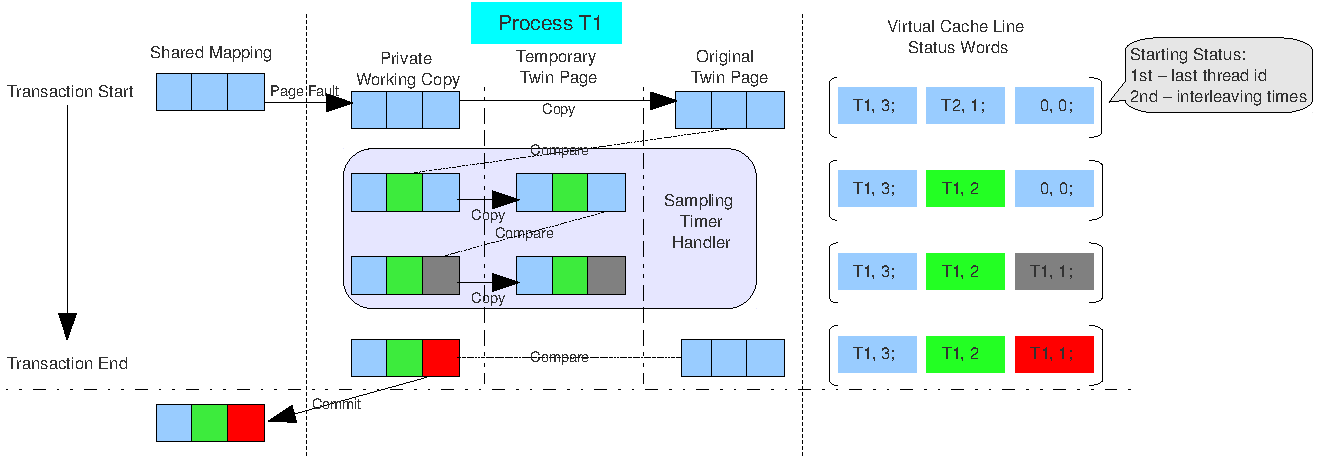
\includegraphics[height=2.3in]{sheriff/figure/overview.pdf}
\caption{
Overview about the execution of Sheriff(Section~\ref{simulation:thread}). 
Sheriff simuates threads using processes(Section~\ref{sec:simulation}). 
Each process works on its private copy  
and commits modifications of current process to shared mapping in the end of transaction(Section~\ref{simulation:endtran})
relying on ``twin page mechanism''(Section~\ref{overview-twinpage}) to get difference. 
To get interleaving writes for detecting false sharing, 
we introduce virtual cache line status words (Section~\ref{detection:invalidation}) 
and sampling mechanism(Section~\ref{detection:sampling}). 
No need for sampling mechanism and status words if only for a runtime system.
\label{fig:overview}}
\end{figure*}

Unlike previous tools, Sheriff is designed based on a completely different approach.
Sheriff doesn't rely on the hardware performance counter or binary instrumentation to find out false sharing problems. 
Alternatively, Sheriff tries to design a runtime system to simulate the running of multi-threaded program and 
monitor memory writes on different virtual cache lines from different threads.
%After the finding of cache lines with numerous interleaving writes,
Sheriff can precisely locate those objects or some fields inside objects causing serious performance problem. 

\subsection{Observations and Targets}
\label{overview:target}
There are two different types of false sharing problems according to 
the definitions of Hyde and Fleisch~\cite{falseshare:Analysis}. 
One is called as ``false sharing'' when multiple structurally unrelated objects 
are located in the same cache line. 
Another is called as ``pseduo sharing'' when multiple processors 
are accessing different fields of the same object.
Sheriff aims to find these two kinds of false sharing problems. 

Note that false sharing not always cause the performance problem. 
Whether one false sharing can cause performance problems depends on memory accessing pattern. 
We observe that false sharing can cause significant performance problems 
only when there are a lot of \textbf{interleaving} memory writes from different threads. 
Based on this observeration, Sheriff is trying to capture interleaving writes from different threads and 
report only those possible false sharing causing performance problem.
%%%%%%%%%%%%%%%%%%%%%%%%%%%%%%%%%%%%%%%%%%%%
%%%%% For global objects, Sheriff can tell the name of global objects which cause the false sharing problems.
%%%%% For heap objects, Sheriff can tell the callsite of malloc, thus programmer can 
%%%% refer to actual source code to find out which object caused the problems.
%%%%%%%%%%%%%%%%%%%%%%%%%%%%%%%%%%%%%%%%%%%%5
%Sheriff won't intend to find instructions that cause false sharing problems. Since multiple 
%instructions located in different functions can cause the same false sharing problem, but without the enough times 
%to capture the attention of programmer.
\begin{comment} 
There are two ways to tell false sharing problems. One is to tell users about the placement to 
touch those false sharing objects. Now PTU can point out functions to access specified addresses, without 
the name of false sharing objects, users should still try to figure out false sharing objects
in the whole function then they can decide how to fix the problem. 
Another is to tell users about false sharing objects, then user can find how false sharing happens.  
\end{comment} 
In order to reduce the manual overhead to locate the root of false sharing problems, Sheriff tries to indentify 
false sharing objects directly. 

Since Sheriff tries to replace those standard pthreads library (including memory allocator) 
in order to avoid the false positive problems 
caused by heap objects, Sheriff can not be used to detect those false sharing problems 
caused by memory allocator. 
We believe that is also reasonable since mordern memory allocator are trying to 
avoid false sharing problems as 
much as possible~\cite{BergerMcKinleyBlumofeWilson:ASPLOS2000}. 
%Section~\ref{effect-application} examplify the easiness to find the root of false sharing problem by using Sheriff.
\subsection{Assumptions}
\label{overview:assumption}
Sheriff has a basic assumption about those evaluating programs 
in order to simulate them correctly using multiprocess mechanism.
Those evaluated program are expected to no synchronization errors, 
such as deadlock, race condition or atomicity violations. 
We believe that this assumption is reasonable. 
If there are some synchronization problems inside, applications running using Sheriff
may have a higher probability to run uncorrectly, which can prevent Sheriff to find out all false sharing problems.

\subsection{Process as Threads}
One basic mechanism of Sheriff is to treat threads as processes, which is used firstly by Grace~\cite{grace}.
%But Sheriff discards the sequential semantics of Grace, which Grace tends to use that to avoid concurrency errors. 
%Also, Sheriff discards the limit of Grace (no synchronization inside) and try to provide a framework
%which can work on general multi-threaded programs. 
Process has its own address space and signal handler table, provides strong isolation between different threads, 
which makes it perfect for Sheriff
to monitor memory accesses from different threads.
More importantly, we can utilize process to eleminate false sharing inside, no need
to let other threads to know results if no explicit synchronization.

There is a natural concern about the performance to use process instead of threads.
Although the overhead to create and exit one process is       
much more than that for one thread, we don't need pay too much overhead here since  
thread's creation and exit won't happen frequently and normal execuation of Sheriff 
can be almost the same speed as that of processes.

Section~\ref{sec:simulation} gives more details about how to simulate threads using process.
\subsection{Twin Page Mechanism}
\label{overview-twinpage}
Sheriff can capture those pages modified by one process 
when one process are trying to write on those pages protected as read-only mode.
But it is clear that page granularity is too coarse to locate cache false sharing problems.  
To avoid this problem, Sheriff are trying to use twin page mechanism to find the modifications on words. 
Twin page mechanism was first used in Munin~\cite{dsm:treadmarks} to 
capture modifications on a page in distributed share memory system.

The mechanism 
can be seen in Fig.~\ref{fig:overview}. 
Before one working page is modified, a ``twin page'' is created which is indentical
to the working page which are going to be modified. The twin page is keeping intact when the working
page are modfied. 
Later, the twin page and the working page can be compared byte by byte
later in order to capture those modifications made on the working page.
\begin{comment}
In the beginning of one synchronization phase, all pages are protected. 
At the first write on one protected page,
a page protection violation occurs. 
Operating system should send a signal handler to current process causing protection violation, 
then in the signal handler Sheriff can makes a copy of current page (creation of a twin page) 
and removes the protection on this page so that future 
writesi (in the same phase) on this page can run at a full speed. 
The twin page and the working copy of current process can be compared word by word
later to capture those writes on this page in one phase.
\end{comment}
More details about using the ``twin page mechanism'' can be seen in Section~\ref{sec:falseshare}.
%In this meaning, we are trying to introduce the "twin" mechanism used in DSM system in a general multithreaded
%program by leveraging constructively the process mechanism in the same time. 


\section{Detecting False Sharing}
\label{sec:falseshare}
From above section, we already know that how to design a runtime system to simulate the running 
of multi-threaded program. 

In this section, we are going to talk how to indentify false sharing problems by recording memory writing using
the runtime system.
This section are trying to answer the following questions:

\begin{itemize}
\item How to capture the memory writes from different process?
\item How to capture the continuous memory writes?
% - sampling mechanism - "temporary twin" and "original twin". 
\item How to capture the interleaving cache invalidation? 
% Use a global array, updating timely when modification is detected. 
\item How to identify objects inside one cache line? 
%Attach the callsite information to capture the allocate sites for heap objects. 
\item How to differentiate true sharing and false sharing?
%detect the combination? An array to get word version and threads working on that. We can detect those fields inside one object causing the problem too.
\item How to report one false sharing problem?
% In the end of program, we traverse the whole global array.
\end{itemize}

\subsection{Capture of Memory Writes}
\label{falseshare:memorywrites}
Process can provide a strong isolation of one thread's running from other threads' running. 
In each transaction, Sheriff runs one thread in a atomical, consistent and isolated way and
won't commit those changes in one transaction until the end of one transaction.
In the end of each transaction, Sheriff can compare ``twin'' page and ``working'' page word by word to find 
those modifications on each dirty page. When the word of ``working'' page is different from that of 
corresponding ``twin'' page, this word is thought to be modified by current thread in current transaction. 
It is reasonable to reach this conclusion since Sheriff can guarantee that originally the content of ``twin'' page 
is the same as that of ``working'' page by forcing a COW explicitely (see ~\ref{simulation:execution}).
\begin{comment}
It is true that the writing of ``A-B-A''  can be missed by simply comparison,
but we believe that ``A-B-A'' writing in one transaction
is not frequent and won't bring any correctness problem.
We don't want to put too much focus on this point.
\end{comment}

Since we can capture the memory writes on every transaction and one thread's running is consisted of multiple transactions, 
we can capture the memory writes from different threads.

\subsection{Capture of Continuous Writes}
\label{detection:sampling}
We already know from above section that Sheriff can capture memory writes on one transaction. 
But it is not good enough when the transaction length is too long (some extreme case can be the whole thread). 
Actually, one serious false sharing problem (\texttt{linear\_regression} benchmark, see Section~\ref{sec:evaluation}) 
which affect the performance 10X can be omitted since there is only one transaction for one thread, 
without any synchronization inside. 

Sheriff use a sampling mechanism to avoid this problem. Sampling is 
to select some of observations in order to acquire some knowledge about the whole.
Although sampling cannot give complete information about memory writes on one transaction,
sampling can be used to capture more writes. More fine sampling can help to find more writes by one transaction.
There is a balance between choosing finer sampling period and performance issue here. 
Sheriff now choose 10 microseconds as a basic interval to do sampling. 

In order to capture continuous writes, Sheriff introduce one ``temporary twin'' page for every shared dirty page
 (see Fig.\ref{fig:overview}). 
Handling of those ``temporary twin'' pages are slightly diferent with those ``original twin'' pages.
First, they are created in the sampling timer handler when one page is found to be shared by multiple threads. 
There is no use to create ``temporary twin'' for those pages only accessed by one thread. We are using a global array to
record users for one page. 
Second, ``temporary twin'' pages are keeping updated to ``working'' version in every timer handler 
in order to capture future writes on the same page.
 
\subsection{Capture of Cache Invalidations}
\label{detection:invalidation}
Just as we talked in Section~\ref{overview:target}, only numerous interleaving writes can bring performance problem. 
Sheriff tries to capture the interleaving writes across different threads in order to capture 
cache invalidations. 

In order to capture interleaving writes on caches, Sheriff introduces 
virtual cache line status words (Fig.~\ref{fig:overview}). 
``virtual'' is used here to differentiate with ``physical'' cache line. 
For every virtual address range (same size with physical cache line) under protection, Sheriff assigns one status word. 
One status word has two fields, the first field points last thread to write on this cache line, 
the second field is used to record times of invalidates (version) on one cache line. 
Every time when one different thread are detected to write on this cache line, Sheriff update both the thread id
to be the new thread and version number. 
In actual implementation, Sheriff introduce two different arrays to avoid using lock. Corresponding code can be seen
in Figure~\ref{fig:capturecacheinvalidation}.
CacheInvalidation array is used to capture those interleaving cache invalidation for all cache lines in protected memory. 
Every cache line have one corresponding counter to indicate the interleaving of cache invalidation for this cache line. 
LastThreadModifyCache array is used to record last thread id to write on its cache line. 

The pseudo code to capture the interleaving cache invalidation is listed in Figure~\ref{fig:capturecacheinvalidation}:
\begin{figure*}[!t]
\begin{lstlisting}
void recordCacheInvalidates(int cacheNo) {
    int myTid = getpid();
    int lastTid;

    // Try to check last thread to modify this cache.
    lastTid = atomic_exchange(&LastThreadModifyCache[cacheNo], myTid);
    if(lastTid != myTid) {
       // Increment cache invalidation only when current thread is different.
       atomic_increment(&cacheInvalidation[cacheNo]);
     }
}
\end{lstlisting}
\caption{Record the cache invalidation atomically.\label{fig:capturecacheinvalidation}}
\end{figure*}

\subsection{Indentify Objects inside Cache Line}
\label{detection:object}
For global object, Sheriff don't need to do anything since debug information can provide
object's information.
Sheriff attaches the call site in the header of each heap object when allocation to indentify objects.
Callsite information can provide objects' request allocation, which is useful for programmer
to fix the false sharing problem (see case study in Section~\ref{evaluation:comparison}).
It is one important feature to differentiate Sheriff from previous tools.
Previous tools using binary instrumentation or hardware performance counter cannot control
the memory allocation, so they cannot provide the callsite information about one object.
Sheriff is a runtime system which intercepts all heap allocations so that Sheriff can tell programmer
about cache line's object information.

Remember that Sheriff have two arrays to capture the cache interleaving invalidation
(see Section~\ref{detection:invalidation}), it is necessary to cleanup those invalid counting
when one object is de-allocated. It is important to avoid the false positives caused by uncorrectly aggregate 
counting when one address is re-used for other objects. 

\subsection{Avoidance of False Positives}
\label{detection:avoidfalsepositive}
To avoid false positives, 
Sheriff introduces another global array to record  
threads writing on each word and version numbers of each word.
Threads writing on each word can tell whether one cache line is false sharing or true sharing. 
Version number on each word can avoid to report those objects which don't contribute much on cache invalidations, 
when there are multiple objects in the same cache line.
In order to save space, Sheriff use one word's higher 16 bit to store the thread id on one word
and use the lower 16 bit to store version number of this word. 
When one word is detected to be modified by more than two threads, we marked specially
on its thread id field.

\subsection{Reporting False Sharing Objects}
In the end of program, Sheriff reports those objects causing false sharing problems. 
Since Sheriff introduce a global array (CacheInvalidationArray) to record those 
cache invalidation (see Section~\ref{detection:invalidation}), Sheriff checks 
CacheInvalidationArray for cache lines with invalidation times larger than one water level. 
After one cache line is found, corresponding invalidation times and offset of this cache line 
will be added into a global link linst sorted by invalidation times. 
Later we can rank the false sharing objects by invalidation times they caused. 

After the traverse of all cache lines, Sheriff tries to get objects information 
for all cache lines in the link list. 
Sheriff uses magic value added in the allocation to differentiate the start of one object. 
Also, the object size information can help to identify the start of one object. 
After finding out those objects inside one cache line, Sheriff should look into the 
array listed in Section~\ref{detection:avoidfalsepositive} to avoid false positives. 

%%%%%%%%%%%%%%%%%%%%%%%%%%%%%%%%%%%%%%%%%%%%%%%%%%%%%%%%%%%%%%%%%%%%%%%%%%%%%
%%%%%%%%%%%%%%%% Where to specify those procedure of timer handler????? LTP
%%%%%%%%%%%%%%%%%%%%%%%%%%%%%%%%%%%%%%%%%%%%%%%%%%%%%%%%%%%%%%%%%%%%%%%


\section{Tolerating False Sharing}
\label{sec:sheriffprotect}
While \SheriffDetect{} can effectively find those false sharing problems of multithreaded programs, it is sometimes difficult or impossible to fix them in order to boost the performance. For example, padding memory to avoid false sharing may even slowdown the performance because of excessive memory consumption or reducing cache utilization~\cite{qinzhao}. Also, time constraints or unavailable source code may prevent the fixes. 

Based on the \sheriff{} framework, we provide the second tool, \SheriffProtect{}, to automatically boost the performance for multithreaded applications with false sharing problems, without programmer intervention.  

\SheriffProtect{} borrows the insight initially introduced by Dubois et.al.~\cite{Dubois:1991:DCE:125826.125941}: {\it delaying updates avoids false sharing}. Because \Sheriff{} replaces threads with processes, executions of different threads are actually isolated from each other. Thus, different ``threads'' (processes) actually access different physical cache lines, when originally they are accessing the same cache line in the multithreading environment. This helps avoid false sharing problems. 

However, simply using \sheriff{} may introduce excessive performance overhead because of the following reasons: 

\begin{itemize}
\item
The overhead of protecting and committing all pages may be too high. As we already know in Section~\ref{sec:sheriffframework}, \sheriff{} has to commit all local changes of different threads  to the shared mapping at the end of every transaction (synchronization points) in order to achieve the shared memory semantics. 

\item
If the length of a transaction is short, the overhead of protecting and committing pages in \sheriff{} can be easily higher than the performance benefit by tolerating possible false sharing problems inside. Thus, there is no benefit to tolerate false sharing problems for short-running transactions. 

\end{itemize}

\sheriffprotect{} provides two corresponding mechanisms to avoid these possible overhead. 

\emph{Selective Protection.} 
\SheriffProtect{} only prevents false sharing on small objects (those less than 1024 bytes in size). All large objects are mapped shared and are never protected, thus can not tolerate false sharing problems caused by these large objects. We expect  small objects to be a likely source of false sharing because more of them can fit on a cache line. Also, for large objects, the cost of protecting and committing changes can be bigger than the benefit of tolerating possible false sharing problems inside. 

\emph{Adaptive Prevention.}
\SheriffProtect{} employs a simple adaptive mechanism: it only isolates threads' executions if the average transaction length is large than a pre-set threshold. \SheriffProtect{} keeps track of the length of each transaction and uses exponential a weighted averaging ($\alpha = 0.9$) to calculate the average transaction length. If the average transaction length falls below an established threshold, \SheriffProtect{} switches to shared mappings for all memory and does no further page protections. As long as transactions remain too short, 
 without any benefit to tolerate false sharing problems inside, the protection mechanisms remain switched off. If the average transaction length rises back above the threshold, \SheriffProtect{} re-establishes private mappings and page protections, thus avoiding possible false sharing to achieve better performance.

\section{Experimental Evaluation}
\label{sec:evaluation}

We perform our evaluations on a quiescent 8-core system (dual
processor with 4 cores), with 8GB of RAM. Each processor is a 4-core 64-bit Intel Xeon, running at 2.33 Ghz with a 4MB L2 cache. For compatibility reasons, we compiled all applications to a 32-bit target using GCC. All performance data is the average of 10 runs, excluding the maximum and minimum values.

The evaluation answers the following questions:

\begin{itemize}
\item How effective is \sheriffdetect{} at finding false sharing and guiding programmers to their resolution? (Section~\ref{sec:effecteval})
\item What is \sheriffdetect{}'s performance overhead? (Section~\ref{})
\item How sensitive is \sheriffdetect{} to different sampling rate? (Section~\ref{}) 
\item How effective does \sheriffprotect{} mitigate false sharing? (Section~\ref{})
\end{itemize}

\subsection{\sheriffdetect{} Effectiveness}

\label{sec:effecteval}

This section evaluates whether \sheriffdetect{} can be used to find false sharing problems, both in synthetic test cases and in actual applications.

We developed a range of microbenchmarks that exemplify different situations related to false sharing. We evaluate these benchmarks on both \SheriffDetect{} and Intel's Performance Tuning Utility(PTU v3.2), the previous state-of-the-art work of false sharing detection.
Detection results are shown in Table~\ref{table:microbenchmarks}. \sheriffdetect{} only reports those false sharing instances that can possibly affect the performance, while correctly ignores those cases without no performance impact.
PTU has false alarms/positives.  It does not track those pattern of accesses, which reports false positives for those non-interleaved accesses. Also, PTU does not track memory deallocations, thus it can not filter out those pseudo false sharing caused by memory reuse. \sheriffdetect{} avoids all of these problems and reports false sharing problems correctly. 


\begin{table}
\centering
\begin{tabular}{l|l|l|l}
\hline
{\bf \small Microbenchmark} & {\bf \small Perf Sensitive } & {\bf \small \sheriffdetect{} } & {\bf \small PTU } \\
\hline

\small \textbf{False Sharing (adjacent objects)} & YES & \cmark{} & \cmark{} \\
\small \textbf{False Sharing (same object)} & YES & \cmark{} & \cmark{} \\
\hline
\small \textbf{True Sharing} & NO & & \\
\small \textbf{Non-interleaved False Sharing} & NO & & \xmark{}\\
\small \textbf{Heap Reuse(no sharing)} & NO & & \xmark{}\\
\hline
\end{tabular}
\caption{False sharing detection results using PTU and \sheriffdetect{}. \sheriffdetect{} correctly reports only actual false sharing instances, with a performance impact;
\cmark{} indicates a correct report and \xmark{} indicates a false alarm. 
\label{table:microbenchmarks}}
\end{table}

We further evaluate \SheriffDetect{} and PTU on two widely-used benchmarks suites, Phoenix~\cite{phoenix-hpca} and PARSEC~\cite{parsec}. We use the simlarge inputs for all applications of PARSEC. For Phoenix, we chose available parameters that allow the programs to run as long as possible. As of this writing, we were unable to successfully
compile \texttt{raytrace} and \texttt{vips}, and \sheriff{} is
currently unable to run \texttt{x264}, \texttt{bodytrack},
and \texttt{facesim}. Freqine currently can not support pthreads. Thus, those benchmarks are excluded here. 
 
\begin{table}
\centering
\begin{tabular}{l|r|r}
\hline
{\bf \small Benchmark} & {\bf \small PTU} & {\bf \small \sheriffdetect{}}\\
 & {\# Lines} & {\# Objects}\\
\hline
\small \textbf{kmeans} & 1916 &  2 \\
\small \textbf{linear\_regression} & 5 & 1 \\
\small \textbf{matrix\_multiply} & 468 & 0\\
\small \textbf{pca} & 45 & 0 \\
\small \textbf{reverseindex} & N/A & 5 \\
\small \textbf{word\_count} & 4 & 3\\
\hline
\small \textbf{canneal} & 1 & 1 \\
\small \textbf{fluidanimate} & 3 & 1 \\
\small \textbf{streamcluster} & 9 & 1\\
\small \textbf{swaptions} & 196 & 0\\
\hline
\small \textbf{Total} & 2647 & 14\\
\hline
\end{tabular}
\caption{Overall detection results of PTU and \sheriffdetect{} on Phoenix and PARSEC benchmark suites. We only list those benchmarks that at least one of tools reports false sharing problems. For PTU, we show how many cache lines are marked as falsely shared. For \sheriffdetect{}, we show how many objects are reported by \sheriffdetect{} (with cache invalidations larger than 100). The item marked as ``N/A'' means PTU fails to show results because it runs out of memory.
\label{table:fsdetection}}
\end{table}


The overall results are shown in Table~\ref{table:fsdetection}. PTU reports that 2647 cache lines may exist false sharing problems, given that they can report false positives. \sheriffdetect{} reveals that seven out of sixteen evaluated benchmarks have some false sharing issues. Totally, only 14 objects are reported, but only 4 of them shows a big number of cache invalidations. 

Several reasons contributes to this big difference. First, PTU reports cache lines information about false sharing objects, while \SheriffDetect{} only reports objects. Second, PTU reports multiple times if a heap object, with the same allocation site, is allocated multiple times. 
Third, PTU may report false positives since it do not track interleaved accesses and overrate the problems caused by heap reuses. 


We manually fix these four false sharing problems based on reports of \SheriffDetect{}, and showed the performance data in Table~\ref{table:perfafterfix}. To explain why performance improvement are different, we examine the maximum possible updates occurred on these false sharing objects, the reason of performance improvement. For example, \texttt{linear\_regression} has the largest updates, thus causes serious performance problem because of false sharing. 

\begin{table}
\centering
\begin{tabular}{l|r|r}
\hline
{\bf \small Benchmark} & {\bf \small Performance Improvement} & {\bf \small Updates}\\
 & & (M)\\
\hline
\small \textbf{linear\_regression} & 818\% & 1323.6\\
\small \textbf{reverseindex} &  2.4\% & 0.4\\
\small \textbf{streamcluster} & 5.4\% & 28.7\\
\small \textbf{word\_count} &  1\% & 0.3\\
\hline
\end{tabular}
\caption{Performance data for four false sharing benchmarks. 
All data are obtained using the standard \pthreads{} library. 
``Updates'' shows how many million updates (in total) occurred on falsely-shared cache lines.
\label{table:perfafterfix}}
\end{table}


In \texttt{reverse\_index} and \texttt{word\_count}, multiple threads repeatedly modify the same heap object. The pseudo code for these two benchmarks are listed in Figure~\ref{fig:reverseindex}. We may use thread-local copy to avoid the false sharing problem here; each thread can modify a temporary variable first and then modify the global \texttt{use\_len} in the end of thread.

\begin{figure}[!t]
\begin{lstlisting}
int * use_len;
void insert_sorted(int curr_thread) {
   ......	
   // After finding a new link
   (use_len[curr_thread])++;
   ......	
}
\end{lstlisting}
\caption{A fragment of source code from \texttt{reverse\_index}. False sharing arises when adjacent threads 
modify the \texttt{use\_len} array. 
\label{fig:reverseindex}}
\end{figure}

\texttt{Linear\_regression}'s false sharing problem is a little different (see Figure~\ref{fig:linear_regression}). 
Two different threads write to the same cache line when the
structure \texttt{lreg\_args} is not cache line aligned. This problem can be avoided easily by padding the structure \texttt{lreg\_args}.

\begin{figure}[!t]
\begin{lstlisting}
struct {
  long long SX;
  long long SY;
  long long SXX;
  ......
} lreg_args;

void *lreg_thread(void *args_in) {
  struct lreg_args * args = args_in;
  for(i = 0; i < args->num_elems; i++) {
    args->SX  += args->points[i].x;
    args->SXX += args->points[i].x 
   	         * args->points[i].x;
  }
  ......	
}
\end{lstlisting}
\caption{A fragment from \texttt{linear\_regression} code. 
Each thread is passed in a different address (\texttt{struct lreg\_args}) and each thread can work on its corresponding \texttt{args\_in}. 
Unfortunately, the size of \texttt{struct lreg\_args} is not cache line aligned (52 bytes) and that
causes two different threads to write to the same cache line simultaneously. 
\label{fig:linear_regression}}
\end{figure}

The false sharing problem detected in \texttt{streamcluster} (one of the PARSEC benchmarks) is similar to the false sharing problem in \texttt{linear\_regression}; two different threads are writing on the same cache line.  In fact, the author tried to avoid the false sharing problems and make every stride a multiple times of cache line size. But the default cache line size is 32 bytes, which is different from the actual physical cache line size that we are used in evaluation (64 bytes).  By simply setting the \texttt{CACHE\_LINE} macro to 64 bytes, it is possible to avoid this false sharing problem completely.


\subsection{Ease of locating false sharing problems}

\noindent
To illustrate how \sheriffdetect{} can precisely locate false sharing problems, we 
use one benchmark (\texttt{word\_count}, a PHOENIX benchmark) as
an example. Our experience with diagnosing other false sharing issues is similar.

Here is an example output from \sheriffdetect{} from \texttt{word\_count}.

\begin{verbatim} 
1st object, cache interleaving writes 
13767 times (start at 0xd5c8e140). 
Object start 0xd5c8e160, length 32. 
It is a heap object with callsite:
callsite0:./wordcount_pthreads.c:136
callsite1:./wordcount_pthreads.c:441
\end{verbatim}

Line 136 (\texttt{wordcount\_\pthreads{}.c}), 
contains the following memory allocation call:

\begin{verbatim}
use_len=malloc(num_procs*sizeof(int));
\end{verbatim}

Grepping for \texttt{use\_len}, a global pointer, quickly leads to this line:

\begin{verbatim}
use_len[thread_num]++;
\end{verbatim}

Now it is clear that different threads are modifying the same object
(use\_len). Fixing the problem by using the
thread-local data copies is now straightforward~\cite{detect:intel}.

By contrast, compare PTU's output in Figure~\ref{fig:wordcount}. Finding this problem is far more complicated with PTU, since it only presents functions using each cache line, not to mention the fact that PTU can
report huge numbers of false positives.  Another shortcoming
of PTU is that ``Collected Data Refs'' number cannot be used as a metric to evaluate the significance of false sharing problems. For this example, PTU only reports 12 references (versus 13767 times for \sheriffdetect{}).

\begin{figure*}[!t]
\centering
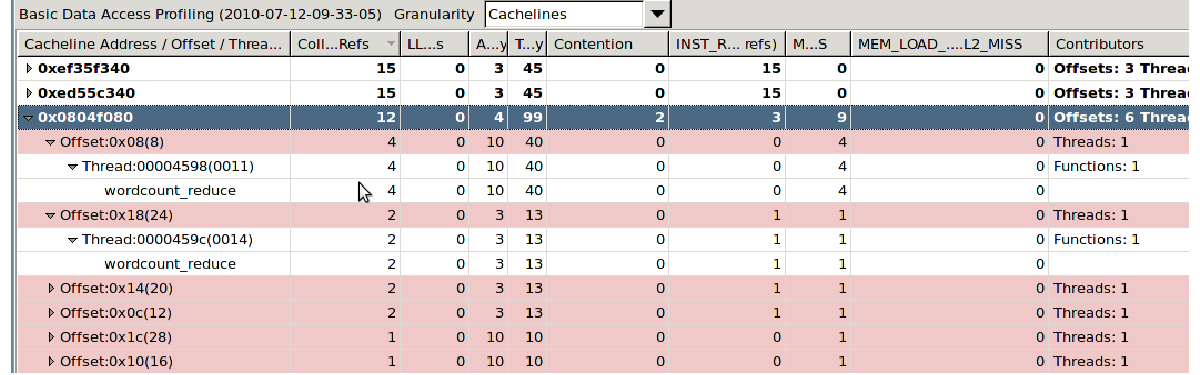
\includegraphics[width=6in]{sheriff/figure/wordcount}
\caption{PTU output for \texttt{word\_count}.
\label{fig:wordcount}}
\end{figure*}

%That is why we cannot relying on PTU to do the analysis of false sharing
%problems given the large number of cache lines involved. 

\subsection{\sheriffdetect{} Performance Overhead}
\label{sec:results-runtime-overhead}

\begin{figure*}[!t]
\centering
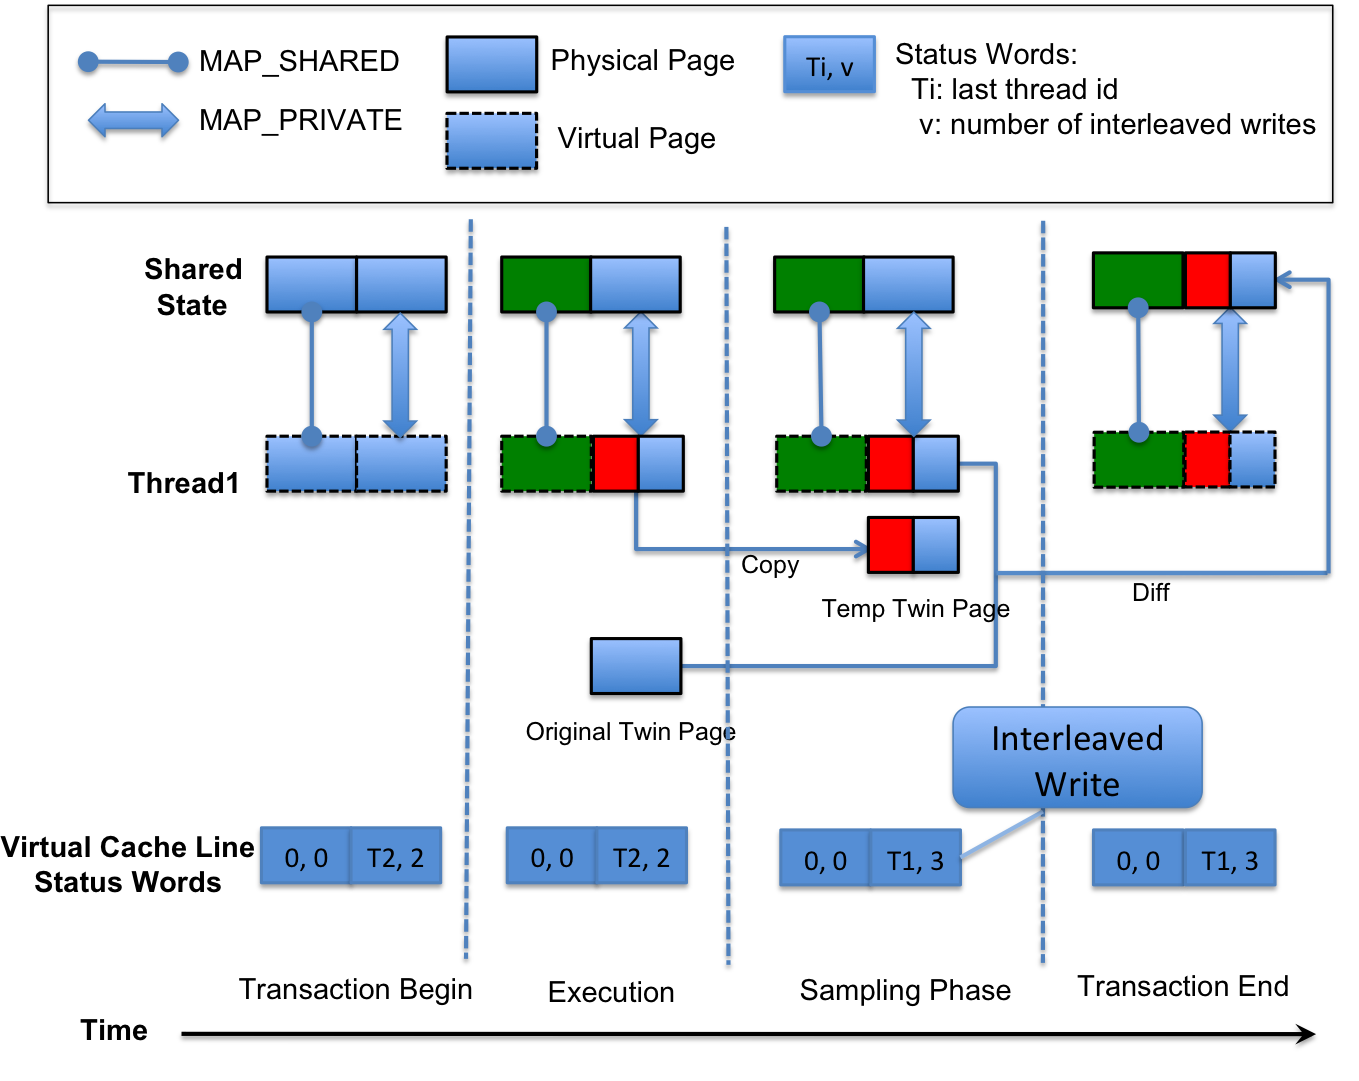
\includegraphics[width=6in]{sheriff/figure/detective.png}
\caption{\sheriffdetect{} overhead across two suites of benchmarks,
  normalized to the performance of the \pthreads{} library (lower is better). 
  With two exceptions, its overhead is acceptably low.
\label{fig:overhead}}
\end{figure*}


This section shows the runtime overhead of \sheriffdetect{} (comparing to \pthreads{})on
two multithreaded benchmarks suites, PHOENIX and PARSEC.  The results
can be seen from Figure~\ref{fig:overhead}.  

\texttt{linear\_regression} exhibits almost
a 10X speedup against the one using \pthreads{} library even with the added overhead of sampling and 
other mechanisms of \sheriffdetect{}.  There is a
serious false sharing problem inside (see
Table~\ref{table:perfafterfix}) which both \sheriffdetect{} and \sheriffprotect{} eliminate
automatically. 

There are two benchmarks on which \sheriffdetect{} do not perform well. 
One is \texttt{canneal}, the performance overhead of \sheriffdetect{}
on this benchmark is about 7X slower than the one using \pthreads{}
library. Another one is \texttt{fluidanimate}, the performance overhead is about 
14X slower than that using \pthreads{}.

According to our analysis, the transaction number and dirty pages are two main causes 
of the overhead. For most of time, more transaction number can cause more dirty pages.  
In order to find out what can affect the performance of these two benchmarks, 
we get some characteristics data(see Table~\ref{tbl:characteristics} about these 
two benchmarks when they are using 
the \sheriffdetect{}.

\begin{table}
\centering
\begin{tabular}{|l|r|r|r|}
\hline
{\bf \small Benchmark} & {\bf \small Trans} &{\bf \small DirtyPages} & {\bf \small Runtime} \\
 & {\#} & {M} & {s}\\
\hline
{\bf \small canneal} & 930 & 2.9 & 74.3 \\
{\bf \small fluidanimate} & 18696114 & 2.15 & 21.56\\
\hline
\end{tabular}
\caption{Characteristics of slower benchmarks in \sheriffdetect{}.
\label{table:characteristics}}
\end{table}

From the table, we can easily find out that these two benchmarks share the same attribute, having large amount of dirty pages. 
For one dirty page, \sheriffdetect{} need two protections, creation of the Copy-On-Write version and
different version of twin pages, checking the false sharing problem inside every periodical checking cycle and 
commits to the shared mapping. Given large amount of dirty pages, copying alone is very expensive 
since one dirty page needs at least 3 copies. 
For \texttt{fluidanimate}, 2.2 million pages needs about 6.8 million copies, which can 
acount for about 20 seconds copying overhead since copying one gigabyte of memory takes approximates 0.75 seconds.
shared pages, which leads to substantial overhead.
Examination of the source code of \texttt{fluidanimate} reveals a large number of lock
calls, \sheriff{} replaces lock calls with their interprocess variants
and triggers a transaction end and begin for each, adding some overhead if there are some shared pages.
 
\begin{comment}
The worst case for \sheriff{} is exemplified
by \texttt{ferret}, which modifies a huge number of pages (about
3.45G) and has a large number of transactions (about 1M).
We also measured charecteristics of our benchmark suites in
Table~\ref{table:characteristics}.  The
following parameters determine the performance of \sheriff{}.

\begin{itemize}
\item
Pages written: each write on a protected page imposes
additional overhead to unprotect the page in the page fault handler.
In the sampling handler, \sheriff{} must check for cache writes for
each shared written page, and at the end of transaction, \sheriff{} must
check cache writes for each page and commit the modification to the shared
space.

\item
Transaction length: \sheriff{} introduces overhead in the beginning
of transaction and in the end of each transaction. Longer transactions
amortizes this overhead.

\item 
Allocation times: \sheriff{} (in detection mode) attaches callsite information for every
allocated object, slowing allocation.

\item
Cache cleanup size: \sheriff{} cleans up the invalid cache counting
information in the memory allocation if one allocation is involving in
the re-usage of memory of those freed memory objects.
\end{itemize}

From the results from Table~\ref{table:characteristics}, we can
confirm our analysis.  Allocation times and cache cleanup size have
little impact on performance. However, when the number and rate of
pages written is large, performance suffers.

Figure~\ref{fig:overhead} shows that \sheriff{}'s overhead is highest for
the following two benchmarks: \texttt{fluidanimate} and \texttt{canneal}.
For \textt{canneal}, different threads are writting to a lot of shared pages
benchmarks \texttt{ferret}, \texttt{reverse\_index}, \texttt{dedup}
and \texttt{fluidanimate}. Characteristics showed in
Table~\ref{table:characteristics} that the first three benchmarks have
a very high rate of page updates (\textbf{PagesPerMs}). 
\texttt{fluidanimate} is an outlier if we are just using the \textbf{PagesPerMs} metrics.
The reason of \texttt{fluidanimate} has a high overhead is that there
are huge amounts of transactions inside (about 10M). Examination of
the source code revealed a large number of lock calls in this
application. \sheriff{} replaces lock calls with their interprocess
variants and triggers a transaction end and begin for each, adding
overhead.  The worst case for \sheriff{} is exemplified
by \texttt{ferret}, which modifies a huge number of pages (about
3.45G) and has a large number of transactions (about 1M).

\begin{table*}
\centering
\begin{tabular}{|l|rrrr|rr|r|}
\hline
{\bf \small Benchmark} & {\bf \small PagesWritten} & {\bf \small Commits} & {\bf Allocs} & {\bf \small CleanupSize} & {\bf \small TranLength(ms)} & {\bf \small PagesPerTran} & {\bf \small PagesPerMs}\\
\hline
\small \textbf{histogram} & 0 & 24 & 2 & 0 & 12.5 & 0 & 0\\
\small \textbf{kmeans} & 1312 & 3836 & 101002 & 0 & 4.15 & 0.34 & 0.08\\
\small \textbf{linear\_regression} & 16 & 24 & 3 & 0 & 38.6 & 0.67 & 0.02\\
\small \textbf{matrix\_multiply} & 16 & 24 & 11 & 0 & 313.23 & 0.67 & 0.0\\
\small \textbf{pca} & 0 & 47 & 2 & 0 & 450.69 & 0 & 0.0\\
\small \textbf{reverseindex} & 260201 & 156409 & 250927 & 0 & 0.05 & 1.66 & 30.99 \\
\small \textbf{string\_match} & 0 & 24 & 7 & 0 & 104.75 & 0 & 0.00\\
\small \textbf{word\_count} & 145 & 89 & 38 & 32 & 25.08 & 1.63 & 0.06\\
\hline
\small \textbf{blackscholes} & 0 & 23 & 4 & 0 & 453.51 & 0 & 0.0\\
\small \textbf{canneal} & 8 & 1056 & 5974612 & 0 & 10.32 & 0.01 & 0.0\\
\small \textbf{dedup} & 76184 & 45636 & 8291 & 0 & 0.04 & 1.67 & 44.9\\
\small \textbf{ferret} & 904381 & 1072258 & 110558 & 0 & 0.01 & 0.84 & 76.04\\
\small \textbf{fluidanimate} & 8 & 10018550 & 135430 & 352 & 0.00 & 0.00 & 0.00\\
\small \textbf{freqmine} & 0 & 1 & 33 & 0 & 11524.6 & 0 & 0.0 \\
\small \textbf{streamcluster} & 32824 & 128557 & 12 & 294 & 0.02 & 0.26 & 10.42\\
\small \textbf{swaptions} & 48 & 24 & 388 & 0 & 167.23 & 2 & 0.01\\
\hline
\end{tabular}
\caption{Characteristics of benchmarks. 
\label{table:characteristics}}
\end{table*}
\end{comment}
%%%%%%%%%%%%%%%%%%%%%%%%%%%%%%%%%%%%%%%5
%%%% Some data to list the effectiveness of this tool.
%%%%%% How many caches are carried for each test case. 
%%%%%% Whether all caches has false sharing problem.
%%%%%%%%%%%%%%%%%%%%%%%%%%%%%%%%%%%%%%%
\subsection{Performance of \sheriffprotect{}}
\label{sec:results-runtime-overhead}

\begin{figure*}[!t]
\centering
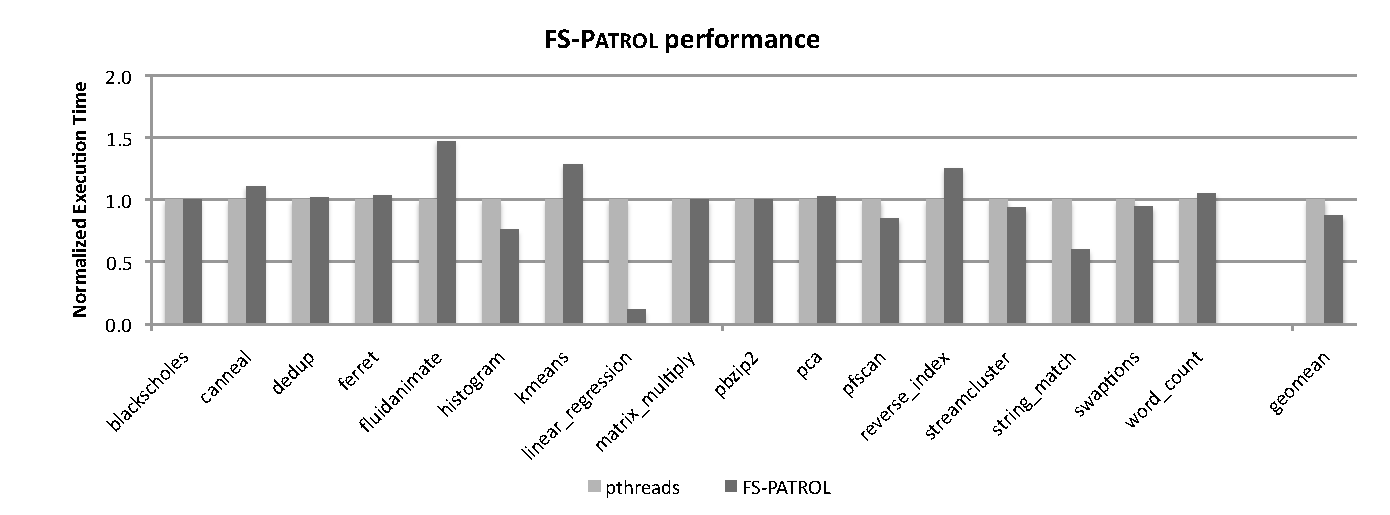
\includegraphics[width=6in]{sheriff/figure/patrolperf.pdf}
\caption{\sheriffprotect{} performance across two suites of benchmarks,
  normalized to the performance of the \pthreads{} library (see
  Section~\ref{sec:results-runtime-overhead}). In case of
  catastrophic false sharing, \sheriffdetect{} dramatically increases performance.
\label{fig:patrol}}
\end{figure*}

Here, we examine the performance improvement by tolerating the false sharing problems in
\sheriffprotect{}.
The performance improvement can be seen in the Figure~\ref{fig:patrol}.  

From the results, we can see that \texttt{linear\_regression} exhibits almost
a 10X speedup against the one using \pthreads{} library.  
By tolerating the serious false sharing problem inside (see
Table~\ref{table:perfafterfix}), \sheriffprotect{} achieves a significant performance 
benefit for this benchmark.
\texttt{histogram} performance benefit comes from one munmap() call to unmap about 400M's file, 
we currently are not sure about why multi-process framework can perform better in this case.

There are three benchmarks which runs at most 30\% slower than using the \pthreads{}. 
We examine the reasons to cause this slowdown. 
For \texttt{kmeans}, this application creates more than 3000 threads about 8 seconds. Since the overhead
to create one process is higher than that to create one thread, this part of 
overhead dominates most of overhead. 

For \texttt{reverse\_index} and \texttt{fluidanimate}, 
they exhibit slowdown because of the use of the processes-as-threads framework. 
This performance impact arises
from the use of a file-based mapping, which connects the private
mapping and shared mapping. The Linux page fault handler does more
work when operating on file-based pages than on anonymous pages (the
normal status of heap-allocated pages). The first write on a
file-mapped page repopulates information from the file's page table
entry. Also, the shared store for all heap pages is initially set to
\texttt{MAP\_SHARED}, so writing to one shared page can cause a
Copy-On-Write operation in the kernel even when there is only one user.
\texttt{fluidanimate} has an enormous number of transactions(18 Million), \sheriffprotect{} 
introduces some additional ovherhead for every trnasaction. That also accounts for part of
overhead.

